%%%%%%%%%%%%%%%%%%%%%%%%%%%%%%%%%%%%%%%%%%%%%%%%%%%%%%%%%%%%%%%%%%%%%%%%%%%%%%%%%%%%
% Do not alter this block (unless you're familiar with LaTeX
\documentclass{article}
\usepackage[margin=1in]{geometry} 
\usepackage{amsmath,amsthm,amssymb,amsfonts, fancyhdr, color, comment, graphicx, environ}
\usepackage{xcolor}
\usepackage{mdframed}
\usepackage{float}
\usepackage[shortlabels]{enumitem}
\usepackage{indentfirst}
\usepackage{physics}
\usepackage{hyperref}
\usepackage{sectsty}
\usepackage{longtable}
\usepackage{complexity}
\sectionfont{\fontsize{12}{15}\selectfont}
\newcommand{\powerset}{\raisebox{.15\baselineskip}{\Large\ensuremath{\wp}}}
\usepackage{tikz}

\usetikzlibrary{arrows,shapes.gates.logic.US,shapes.gates.logic.IEC,calc,decorations.pathmorphing}
\tikzset{snake it/.style={decorate, decoration=snake}}

\usepackage{subcaption}
\usepackage{amsfonts}
\usepackage{lipsum}
\usepackage{setspace}
\usepackage[qm]{qcircuit}
\usepackage[mmddyy]{datetime}
\usepackage{mathtools}
\DeclarePairedDelimiter\ceil{\lceil}{\rceil}
\DeclarePairedDelimiter\floor{\lfloor}{\rfloor}
\usepackage{tkz-euclide}
\usepackage{wasysym}
\hypersetup{
    colorlinks=true,
    linkcolor=blue,
    filecolor=magenta,      
    urlcolor=blue,
}


\makeatletter
\renewcommand*\env@matrix[1][*\c@MaxMatrixCols c]{%
  \hskip -\arraycolsep
  \let\@ifnextchar\new@ifnextchar
  \array{#1}}
\makeatother

\definecolor{lightgray}{rgb}{0.83, 0.83, 0.83}
\pagestyle{fancy}

\def\centerarc[#1](#2)(#3:#4:#5)% Syntax: [draw options] (center) (initial angle:final angle:radius)
    { \draw[#1] ($(#2)+({#5*cos(#3)},{#5*sin(#3)})$) arc (#3:#4:#5); }

\newcommand*\unit[1]{\mathbf{\hat{{#1}}}}

\newcommand\avg[1]{\langle #1 \rangle}

\newenvironment{problem}[2][Problem]
    { \begin{mdframed}[backgroundcolor=gray!20] \textbf{#1 #2} \\}
    {  \end{mdframed}}

% Define solution environment
\newenvironment{solution}{\noindent \textbf{Solution}\\}

% \begin{mdframed}[backgroundcolor=gray!20, align = center, userdefinedwidth = 3.8in]
%     \includegraphics[width = 3.5in]{5C_HW5_Img2.png}
% \end{mdframed}

    
%%%%%%%%%%%%%%%%%%%%%%%%%%%%%%%%%%%%%%%%%%%%%
%Fill in the appropriate information below 
\lhead{Thomas Lu}
\chead{\textbf{Signal Generator Notes}}
%%%%%%%%%%%%%%%%%%%%%%%%%%%%%%%%%%%%%%%%%%%%%


\begin{document}
    \section*{Fri 2/23}
    \subsection*{Function generator general exploration}
    Using the built-in controls of the function generator (AFG), I generated waveforms using the built-in menu options (e.g. sine, square, pulse,) and displayed the signals on the oscilloscope. I also familiarized myself with the various functions and controls on the oscilloscope and AFG.
    \subsubsection*{Phase difference due to cables}
    Both channels on the AFG were set to 6MHz, 200m$V_{pp},$ with a phase offset of $0,$ and were connected to channels 1 and 2 on the oscilloscope. Even after the "Align Phase" option on the AFG is enabled, the oscilloscope still shows a slight phase difference: 
    \begin{mdframed}[backgroundcolor=gray!20, align = center, userdefinedwidth = 3.8in]
    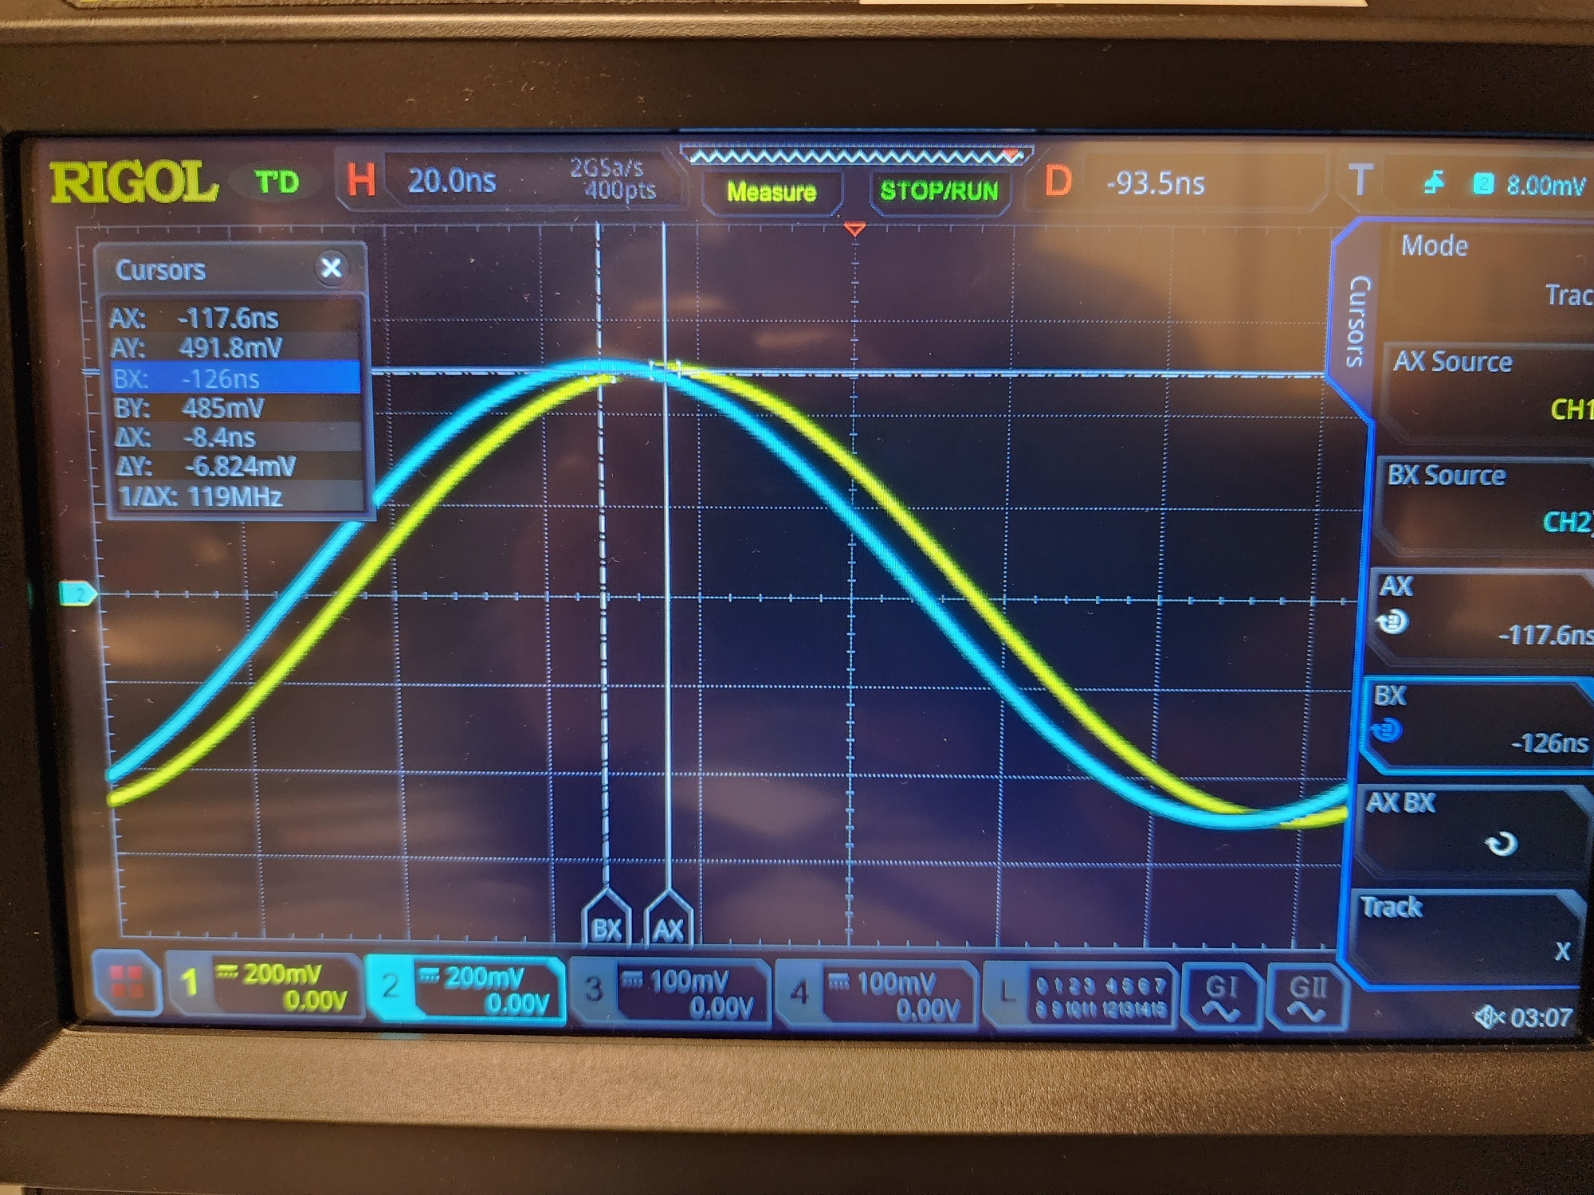
\includegraphics[width = 3.5in]{img/phase_difference.jpg}
    \\Peak-to-peak difference of 8.4ns between CH1 (yellow) and CH2 (blue)
    \end{mdframed}
    This could be due to the difference in wire lengths, as the CH2 wire was 70cm, while the CH1 wire was 210cm long. We can use this to very roughly calculate the speed of the signal:
    $$v = \frac{\Delta \ell}{\Delta t} = \frac{140cm}{8.4ns} \approx 0.55c$$
    which seems reasonable for electrons in copper wire. \textbf{TODO: get two cables of the same length and verify that the phase lag goes away.}
    \subsection*{Programming the function generator with a computer (LAN)}
    Useful resources:
    \begin{itemize}
    \item \href{https://acidbourbon.wordpress.com/2019/09/12/send-numpy-data-to-rigol-dg4202-arbitrary-waveform-generator-via-lan/}{Example using LAN and Python}
    \item \href{https://www.eevblog.com/forum/testgear/dg4000dg4162-scpi-arbitrary-waveform-programming/}{General info about programming}
    \item \href{https://www.eevblog.com/forum/testgear/dg4000-a-firmware-investigation/}{Deeper dive into firmware}
    \item Programming Reference: \textbf{DG4000\_ProgrammingGuide\_EN.chm} (in the repo)
    \item \href{https://download.rigol.com/cn/Software/UltraSigma.zip}{Download Ultra Sigma Software}
    \end{itemize}
    A script for sending a waveform to the AFG via LAN can be found in the Python file \textbf{LAN\_waveform\_test.py}, and follows the tutorial in the first link\\\\
    Setup: Connect the AFG to the computer by Ethernet, go to Utility $\to$ I/O $\to$ LAN and ensure the IP address matches the one in the script. Then, use the script to specify the desired waveform functions, frequency, and voltage range.
    \begin{mdframed}[backgroundcolor=gray!20, align = center, userdefinedwidth = 5.8in]
    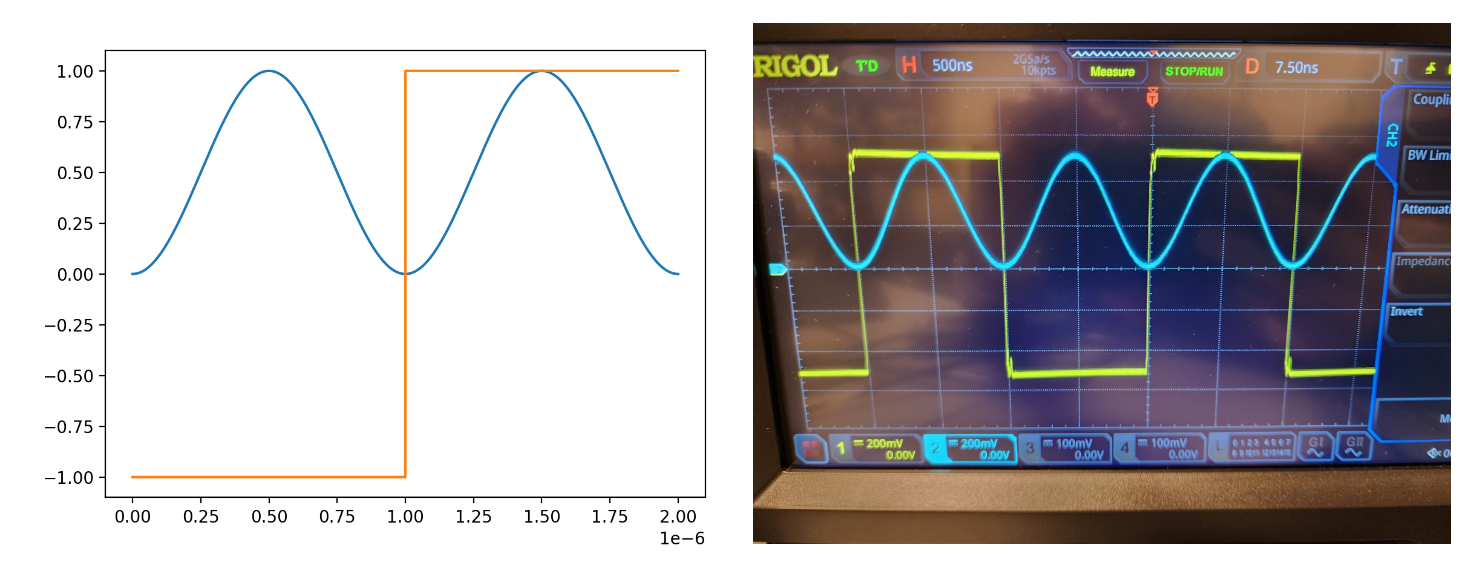
\includegraphics[width = 5.5in]{img/LAN_signal.png}
    \\Left: plot of waveform made with plt; Right: waveform on oscilloscope. Waves are $\sin^2(x)$ (blue) and step function. 500kHZ, 1$V_{pp}$.
    \end{mdframed}
    \subsection*{Ultra Sigma Software}
    The built-in software provided by Rigol is Ultra Sigma. The features when connecting with LAN seem redundant, as it only gives access to the same SCPI commands that we previously sent using the Python interface, and has no way of interfacing with NumPy or external files.
    \begin{mdframed}[backgroundcolor=gray!20, align = center, userdefinedwidth = 4.8in]
    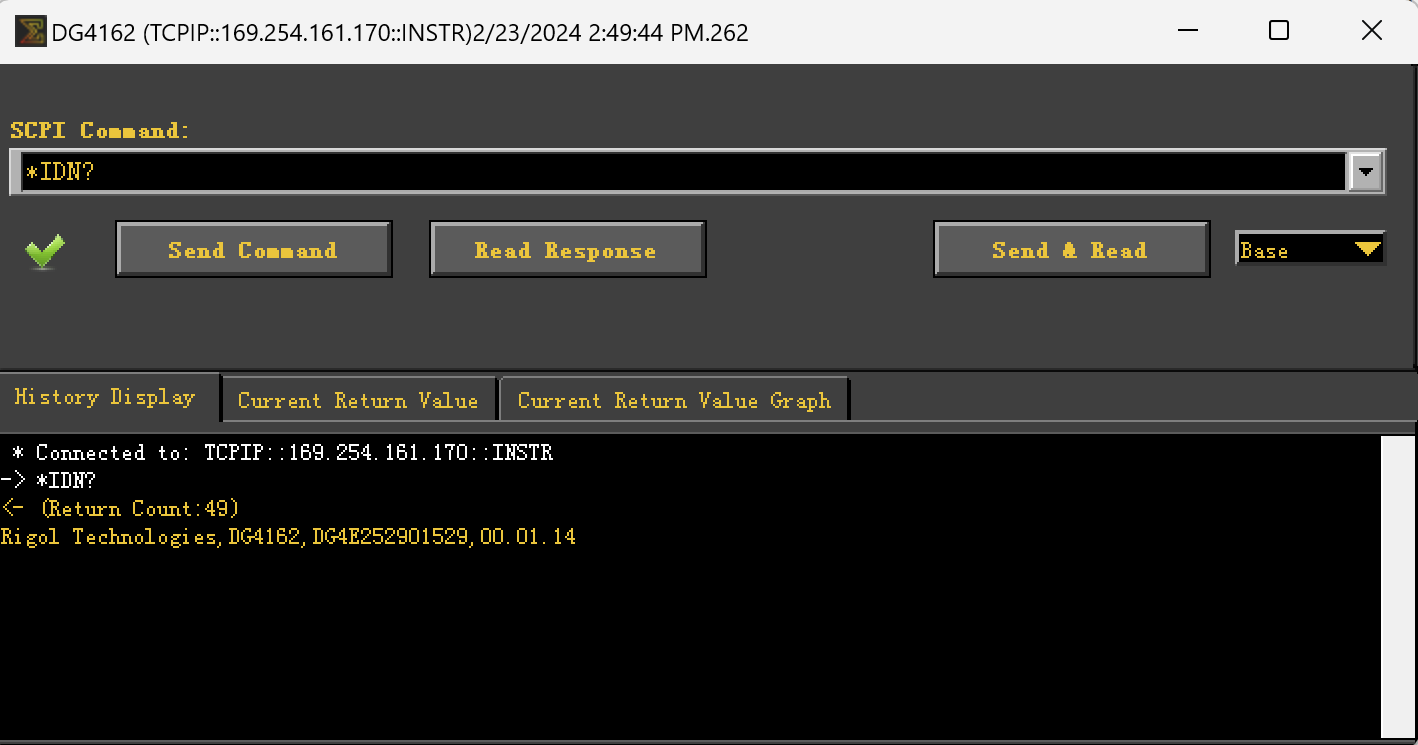
\includegraphics[width = 4.5in]{img/ultraSigmaInterfaceLAN.png}
    \\Ultra Sigma LAN interface
    \end{mdframed}
    Connecting via the USB-B port on the back of the AFG yields the same interface. There is the Ultra Station software that offers more tools for making waveforms, but it is paid and requires a licence. Therefore, LAN/python seems like the best approach moving forward unless we need any advanced features that cannot be reasonably implemented in that approach.
    \section*{Fri 3/1}
    \subsection*{Verifying phase difference from last time due to cables}
    We further test the hypothesis that the difference in cable lengths produced the phase lag observed last time. A new cable of length 210cm was obtained, and the same AWG settings were used (6MHz, 200m$v_{pp}$, $0^\circ$ start phase). Then, we verify that there is no longer any phase difference after "Align Phase" is used on the AWG:
    \begin{mdframed}[backgroundcolor=gray!20, align = center, userdefinedwidth = 4.8in]
    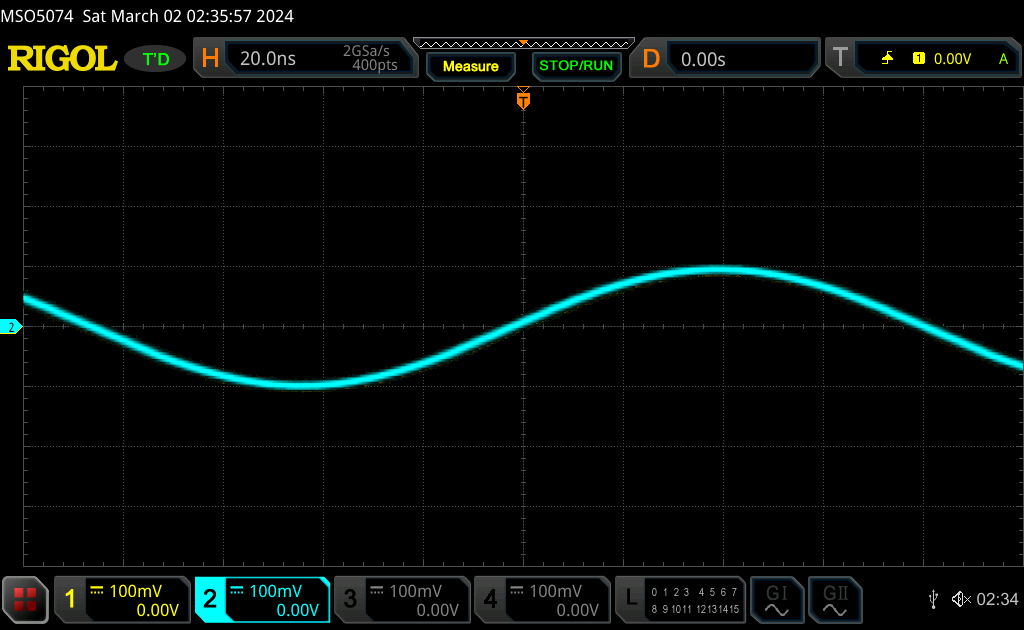
\includegraphics[width = 4.5in]{img/CableLagFixed.png}
    \\No visible peak-peak difference after 210cm cables are used for both channels; data collection via USB drive
    \end{mdframed}
    Therefore, we get further verification of the hypothesis from 2/23 that the phase lag was due to the difference in cable lengths.
    \subsection*{Triggering}
    General settings for oscilloscope: N Cycle burst, 1MHz, $200mV_{pp}.$ For burst, Cycles = 500,000 which means the total pulse duration is $0.5s.$ $N$ can be set arbitrarily, so it is also possible to set smaller numbers of waves to be generated in each pulse, (i.e. a single wave per pulse), depending on the application.\\\\
    Manual trigger: A pulse is generated each time the Trigger button on the oscilloscope is pressed.\\\\
    External trigger using the signal generator on the oscilloscope: Connect $G1$ on the oscilloscope to the [Mod/FSK/Trig] connector on the back of the oscilloscope. Then, set G1 to the following settings: [Ramp waveform, 1Hz, 5$V_{pp}$]. \textbf{TODO: DG4000 manual suggests using a TTL pulse to trigger but the oscilloscope can only generate Ramp waveforms, figure out if there's a difference.}\\\\
    \textbf{TODO: Get a signal splitter to visualize the trigger waveform on the oscilloscope.} Current (somewhat questionable) workaround: set G2 on the oscilloscope to the same waveform settings as $G1$ and align phase for an (approximate) visual reference.
    \begin{mdframed}[backgroundcolor=gray!20, align = center, userdefinedwidth = 4.8in]
    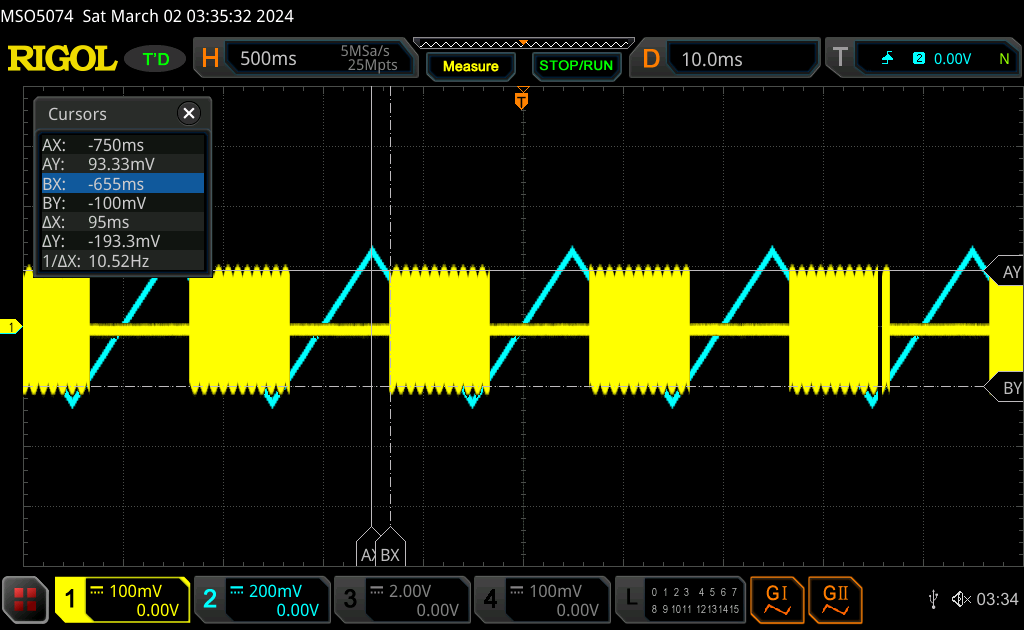
\includegraphics[width = 4.5in]{img/TriggerTest1.png}
    \\Approx. 95ms lag between trigger point (trailing slope) and the start of the burst.
    \end{mdframed}
    We see that there is a 95ms delay between the start of the trigger point (trailing slope) and when the signal is actually received by the oscilloscope. Note that the "Delay" option on the AWG is set to 0, so the delay seems to be intrinsic to the system.\\\\
    Test 2: Higher triggering frequency: Set Cycles = 5000 (5ms pulse), trigger frequency to $100Hz$. We still see a lag, which is $1ms$ this time.\\\\
    \begin{mdframed}[backgroundcolor=gray!20, align = center, userdefinedwidth = 4.8in]
    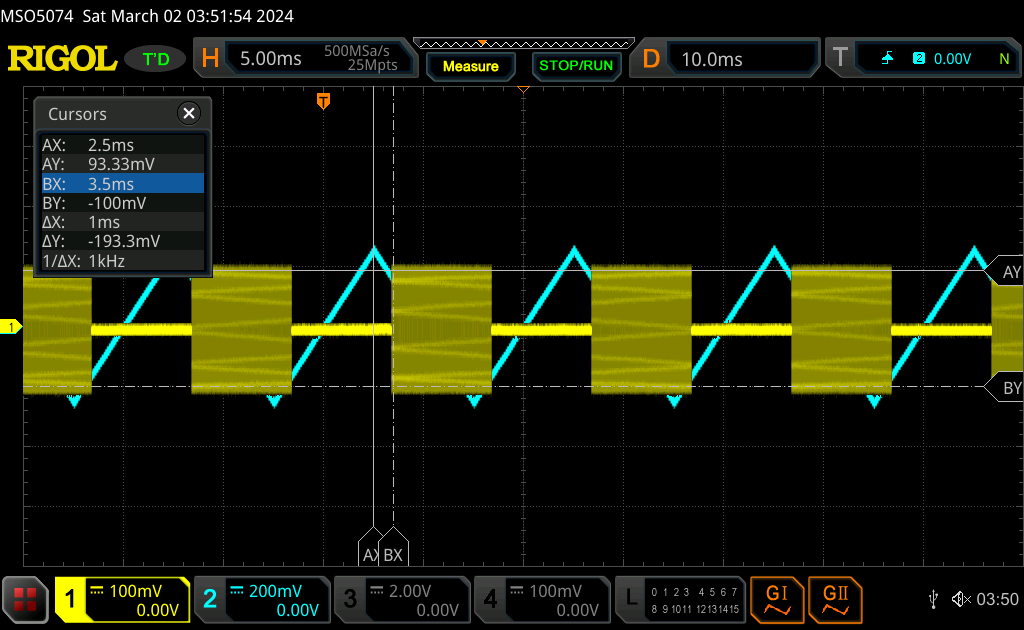
\includegraphics[width = 4.5in]{img/TriggerTest2.png}
    \end{mdframed}
    Test 3: Even higher frequency: Cycles = $5$ (5$\mu s$ pulse), trigger frequency to $100KHz$. The scope seems slightly unstable (waveforms are wobbling slightly - which could be due to triggering settings, etc (trigger based on the $G1$ function from the oscilloscope). However, the waveforms are still well-formed, and there is a delay of $1.27 \mu s$
    \begin{mdframed}[backgroundcolor=gray!20, align = center, userdefinedwidth = 3.8in]
    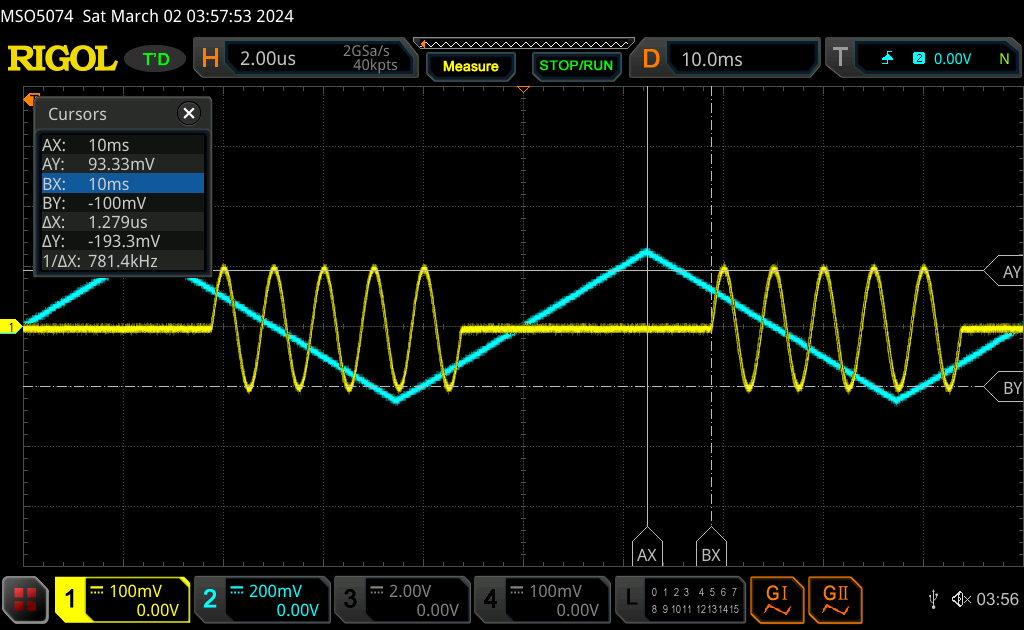
\includegraphics[width = 3.5in]{img/TriggerTest3.png}
    \end{mdframed}
    Conclusions: Triggering using the AWG output from the oscilloscope produces a clean signal for trigger/pulse frequencies of up to 100 $KHz,$ which was the highest trigger frequency tested. Using the ramp waveform to trigger, there appears to be a delay between the start of the trigger and the waveform being produced, of roughly $\frac{1}{10}T,$ where $T$ is the period of the trigger.
    \subsubsection*{Hypothesis}
    Hypothesis: This is due to the oscilloscope needing time to detect the falling edge on the ramp waveform, so this could be fixed if a more appropriate trigger waveform was selected (e.g. TTL). However, it is natural to expect some delay due to factors intrinsic to the system, and in any case it should be possible to calibrate out the delay.
    \subsubsection*{Further Experiments with a square wave}
    A square wave has a much faster drop-off, so would it decrease the latency? 
    \begin{mdframed}[backgroundcolor=gray!20, align = center, userdefinedwidth = 3.8in]
    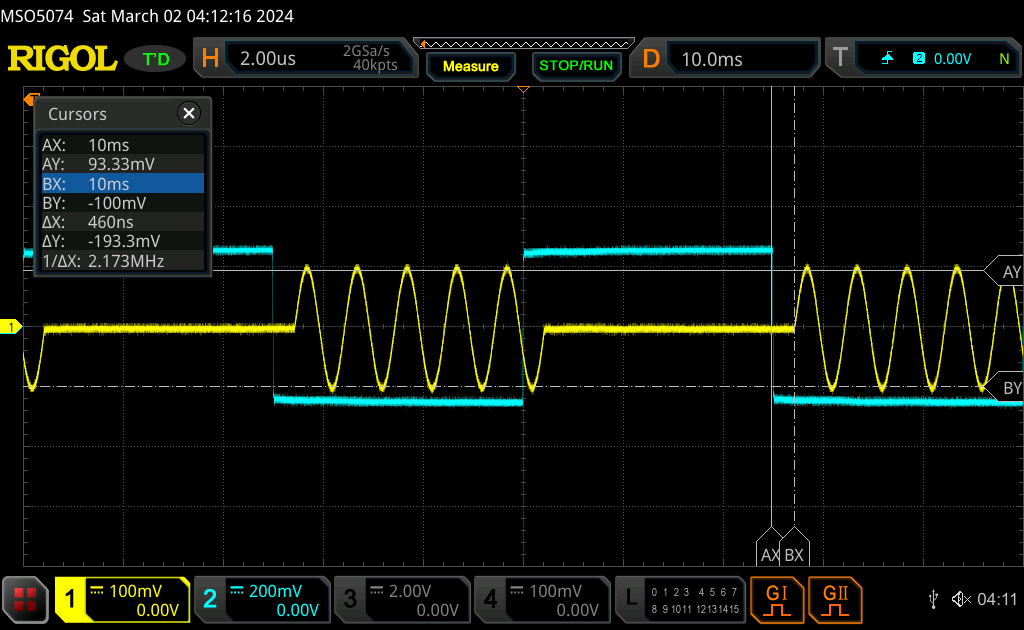
\includegraphics[width = 3.5in]{img/TriggerTestSq.png}
    \end{mdframed}
    \begin{table}[H]
    \centering
    \begin{tabular}{|l|l|l|l|}
    \hline
    Signal Freq & 1Hz & 100Hz & 100KHz \\ \hline
    Ramp Delay & 95ms & 5ms & 1.3 $\mu s$ \\ \hline
    Square Delay & $\sim 0.5 \mu s$ & $0.4 \mu s$ & $0.46 \mu s$ \\ \hline
    \end{tabular}
    \end{table}
    Conclusion: there is approx. $0.4\mu s$ intrinsic delay between the triggering signal and the waveform being generated, and the delay from before was due to the ramp wave.
    \newpage
    \subsection*{Writing Arbitrary Functions, Windowing, Spectral Analyzer}
    Friday Afternoon: spectral analyzer could not be located, so instead logged data from the oscilloscope and used SciPy Fourier transform.
    \subsubsection*{First proof of concept}
    \noindent Let us begin by defining a wave
    $$A(x) = \sin(50(2\pi x)) + \sin(80(2\pi x)),$$
    and consider a sample in $x \in [0, 3/4].$ Because the sample is limited to an interval, it is implicitly windowed with an uniform window function ($A(x) = 0$ for $x \notin [0, 3/4]$). We can also consider the same sample but explicitly windowed with a Blackman window function:
    \begin{mdframed}[backgroundcolor=gray!20, align = center, userdefinedwidth = 4.8in]
    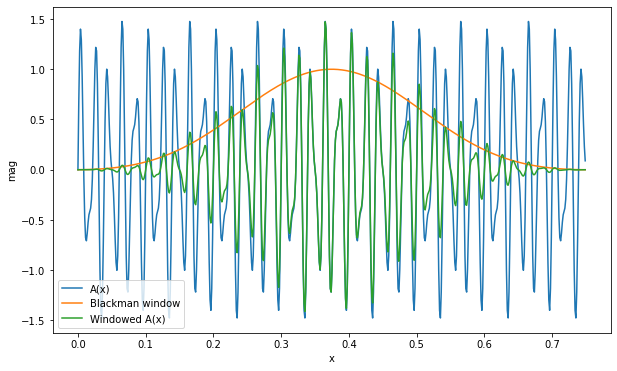
\includegraphics[width = 4.5in]{img/window_function_plot.png}
    \end{mdframed}
    We can see that the spectral leakage is significantly lower with the Blackman window function:
    \begin{mdframed}[backgroundcolor=gray!20, align = center, userdefinedwidth = 3.8in]
    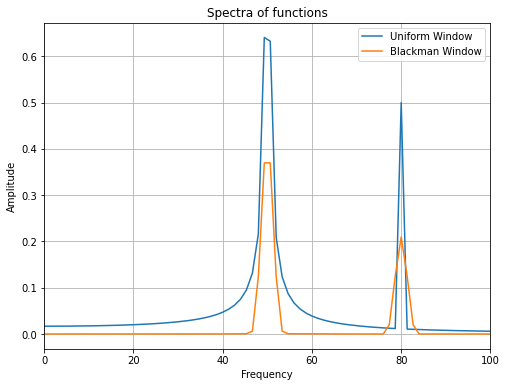
\includegraphics[width = 3.5in]{img/WindowedLeakage.png}
    \end{mdframed}
    \newpage
    \section*{Monday 3/4}
    \subsection*{Spectrum Analyzer}
    The spectrum analyzer could not be located on Monday afternoon.
    \subsection*{Sending Windowed Function to the AWG}
    Now, we proceed to test this using the AWG and oscilloscope. Using the code from before to send the function to the AWG, we pre- and post-pad the waveform with an equal length of zeroes.
    \begin{mdframed}[backgroundcolor=gray!20, align = center, userdefinedwidth = 4.8in]
    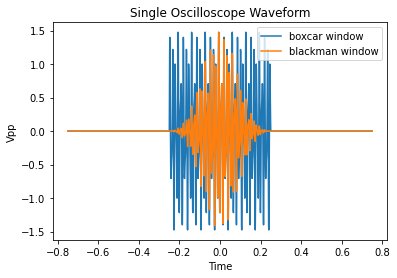
\includegraphics[width = 4.5in]{img/oscilloscope waveform.png}
    \end{mdframed}
    The waveforms are then sent to the oscilloscope with frequency 50KHz and amplitude $3V_{pp},$ and data is collected from the oscilloscope as a CSV file. Then, the time axis is multiplied by $50*10^3$ so that the frequencies of the data are the same as those shown on the previous page.
    \begin{mdframed}[backgroundcolor=gray!20, align = center, userdefinedwidth = 4.8in]
    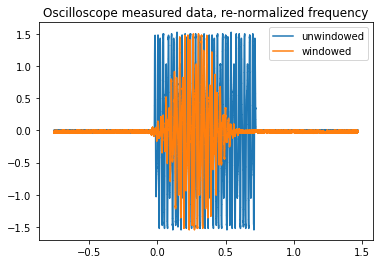
\includegraphics[width = 4.5in]{img/oscilloscopeOut.png}
    \end{mdframed}
    When we compute the Fourier transform using numpy, we see that the windowed waveform shows less spectral leakage, which is the same result as in the simulation from before.
    \begin{mdframed}[backgroundcolor=gray!20, align = center, userdefinedwidth = 4.8in]
    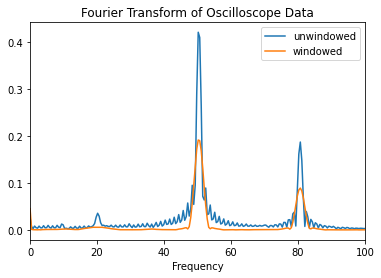
\includegraphics[width = 4.5in]{img/oscilloscopeTransform.png}
    \end{mdframed}
\end{document}